\clearpage
\section{Secure Multi-Party Computation}

\begin{refsection}

\begin{tcolorbox}	
\begin{tabular}{p{2.75cm} p{0.2cm} p{10.5cm}} 	
\textbf{Students Name}      &:& Mariana Ramos (02/05/2018 - 21/05/2018) \\
\textbf && Goncalo Vitor (15/06/2018 - x)\\
\textbf{Goal}               &:& Description of the problem of Secure Multi-Party Computation.\\
\textbf{Directory}          &:& \\
\end{tabular}
\end{tcolorbox}


\subsection{Problem definition}

In \textit{Secure Multi-Party Computation} (SMC) the function to be computed is defined as $(y_1,y_2,...,y_N)=f(x_1,x_2,...,x_N)$ and each party $i$ must only know (before and after the computation) its $x_i$ and $y_i$ being unknown any information about the input or output of the other parties. \cite{Naumann16}.

Thus, there are two ways of solving the problem of SMC:

\begin{enumerate}
  \item The result can be computed using a trusted party involved who has the trust from all the parties. This is a simple solution for the current problem, however, it requires a trusted party.
  \item The result can be computed without a trusted party involved using a SMC protocol. We are going to consider the \textit{Garbled Circuit Protocol} (GCP), which will have our best attention in this chapter.
\end{enumerate}

We will only focus on a two-party computation ($N=2$), with a single output, i.e. $y = f(x_1, x_2)$.

\subsection{Secure Two-Party Computation}

The \textit{Garbled Circuit Protocol} (GCP) starts with a transformation of the $f(x_1,x_2,...,x_N)$ function into a boolean circuit. The logical function $f_c$ is the output of the logical boolean circuit generator which implements $f(x_1,x_2,...,x_N)$. From the logical implementation, $f_c( )$, Alice will generate a garbled version of the logical function, $F_g^f$, as well as an encryption key $e_g^f$ and a decryption key $d_g^f$. After that, Alice's input parameter ($x_1$) and Bob's input parameter ($x_2$) must both be encrypted using the key $e_g^f$. Note that the encryption must be implemented with OT because Alice cannot know the Bob's input $x_2$ and Bob cannot know the encryption key, $e_g^f$, generated by Alice \cite{Naumann16}. Therefore after encryption Bob only gets $X_2$, which is its garbled input parameter. Next, Alice sends to Bob the garbled circuit, $F_g^f$, and its garbled input, $X_1$. With $F_g^f$, $X_1$ and $X_2$ Bob computes, the garbled output $Y_g^f$. With $Y_g^f$ and the decryption key $d_g^f$, Bob obtains $y=f(x_1,x_2)$. To conclude the protocol Bob will send to Alice the result $y$. Figure \ref{fig:garbledcircuit} shows the diagram of \textit{garbled circuit protocol}.

\begin{figure}[H]
	\centering
	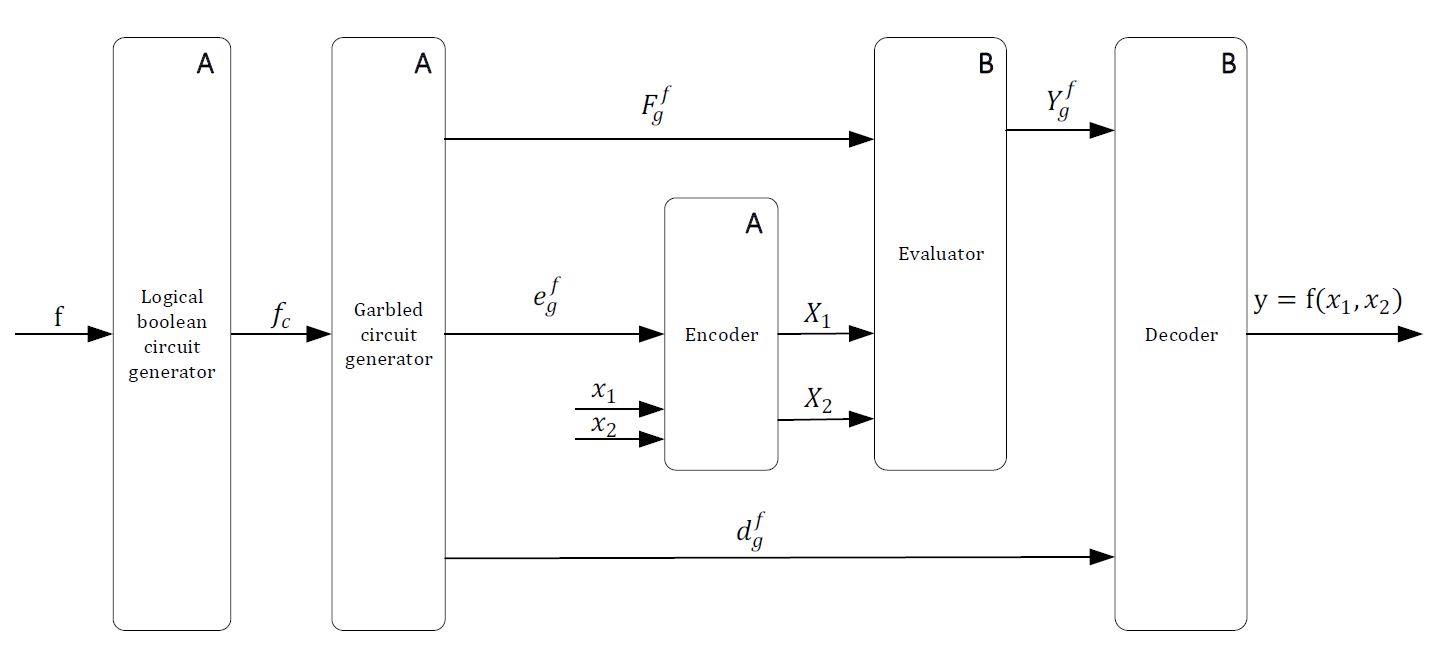
\includegraphics[width=1\textwidth, height=7cm]{./sdf/secure_multiparty_computation/figures/garbled_circuit.png}
    \caption{Block diagram of the garbled circuit protocol. Function to be computed $y=f(x_1, x_2)$. The blocks with label A are implemented by Alice and the blocks with label B are implemented by Bob.}\label{fig:garbledcircuit}
\end{figure}


\begin{table}[H]
\centering

\begin{tabular}{|c|c|}
\hline
$x_1$                   & Alice input parameter             \\ \hline
$x_2$                   & Bob input parameter               \\ \hline
$f$                     & Function to compute               \\ \hline
$f_c$                   & Logical function to be computed   \\ \hline
$F_g^f$                 & Garbled circuit of $f$            \\ \hline
$X_1$                   & Alice garbled input               \\ \hline
$X_2$                   & Bob garbled input                 \\ \hline
$e_g^f$                 & Encoding key                      \\ \hline
$d_g^f$                 & Decoding key                      \\ \hline
$Y_g^f$                 & Garbled output                    \\ \hline
\end{tabular}
\caption{Description of parameters of figure \ref{fig:garbledcircuit}.}
\end{table}




\subsubsection{Example of a two-party computation with a single output}

Lets assume:

\begin{equation}\label{eq:f_to_be_computed}
  y=f(x_1,x_2),
\end{equation}
with,

\begin{equation}\label{eq:fc_to_be_computed}
  y=f_c(x_1, x_2) = x_1 \wedge x_2,
\end{equation}
where $x_1$ and $x_2$ are single bit values. Note that even if the input parameters of $f$ and $f_c$ are represented by the same symbols they are different. The input parameters of $f_c$ are logical representations of the input parameters of $f$.

\begin{figure}[H]
	\centering
	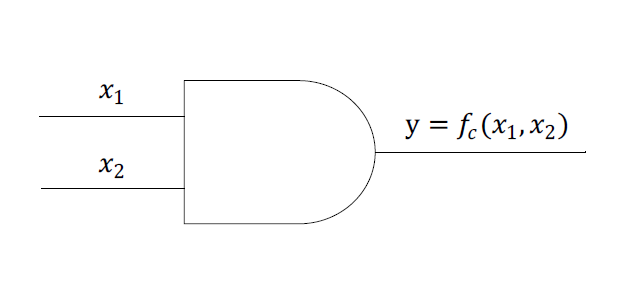
\includegraphics[width=0.4\textwidth, height=2.5cm]{./sdf/secure_multiparty_computation/figures/Gate.png}
    \caption{Gate level implementation of $f_c$.}\label{fig:andGate}
\end{figure}

Figure \ref{fig:andGate} shows the logical boolean circuit representation of the function to be computed. In this particular case there are two parties, each with an input parameter $x_i$, where $i$ can be $1$ (Alice) or $2$ (Bob), and $x_i$ can take values $0$ or $1$. Alice will play the role of \textit{garbled circuit generator} so she will generate a garbled AND gate and send it to Bob. On the other hand, Bob will play the role of \textit{garbled circuit evaluator}.

\begin{figure}[H]
	\centering
	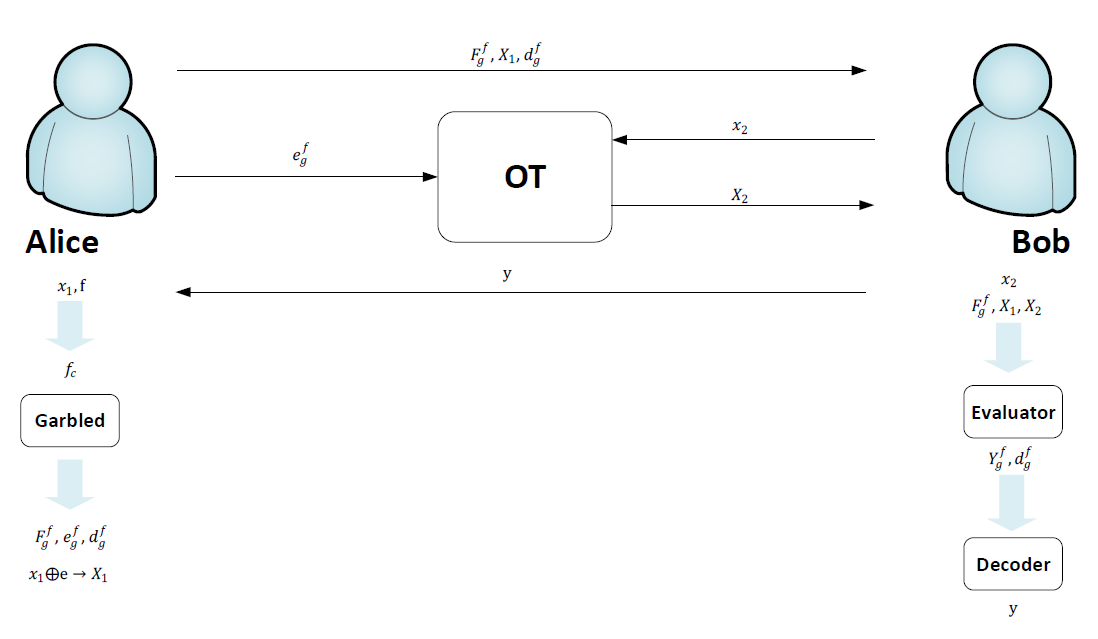
\includegraphics[width=1\textwidth, height=10cm]{./sdf/secure_multiparty_computation/figures/smc_with_ot.png}
    \caption{Garbled Circuit Protocol with OT.}\label{fig:smcwithot}
\end{figure}



\begin{table}[H]
\centering
\begin{tabular}{|c|c|c|}
\hline
$x_1$           & $x_2$             & $y=x_1 \wedge x_2$       \\ \hline
0               & 0                 & 0                             \\ \hline
0               & 1                 & 0                             \\ \hline
1               & 0                 & 0                             \\ \hline
1               & 1                 & 1                             \\ \hline
\end{tabular}
\caption{Truth table of $f_c(x_1,x_2)$.}\label{tb:truthtable}
\end{table}

Table \ref{tb:truthtable} shows the truth table of $f_c$.

Initially, Alice generates an encryption key with length equals to the sum of the length of both input parameters, two bit length in this case. Then, she encrypts her two possible input parameters, $X_1 = x_1 \bigoplus e_g^f[1]$, as well as Bob's two possible input parameters, $X_2 = x_2 \bigoplus e_g^f[2]$. 

Lets assume $e_g^f = 01$ the encryption key used by Alice. In this case, the encryption key has two bits and Alice will use the first bit to encrypt her input parameter $x_1$ and the second bit to encrypt Bob's input parameter $x_2$. We are defining the Alice encrypted input value with the label $W_1^0$ when it before encryption assumes the value $x_1 = 0$, and $W_1^1$ when it before encryption assumes the value $x_1 = 1$. The same happens for Bob, please see table \ref{tb:aliceinputs} and \ref{bobinputs}.
Now, Alice performs the encryption operation for each $x_i$, where $i \in\{1,2\}$. Regarding with Alice's input parameter, where $i=1$:

\begin{table}[H]
\centering
\begin{tabular}{|c|c|}
\hline
$x_1$           & $X_1 = W_1^{x_1}$                             \\ \hline
0               & $W_1^0=x_1 \bigoplus e = 0$                   \\ \hline
1               & $W_1^1=x_1 \bigoplus e = 1$                   \\ \hline
\end{tabular}
\caption{Encryption results for Alice's input parameter $x_1$ using the first bit of encryption key $e[1]=0$.} \label{tb:aliceinputs}
\end{table}
and regarding with Bob's input parameter $x_2$:

\begin{table}[H]
\centering
\begin{tabular}{|c|c|}
\hline
$x_2$           & $X_2 = W_2^{x_2}$                             \\ \hline
0               & $W_2^0=x_2 \bigoplus e = 1$                   \\ \hline
1               & $W_2^1=x_2 \bigoplus e = 0$                   \\ \hline
\end{tabular}
\caption{Encryption results for Bob's input parameter $x_1$ using the second bit of encryption key $e[2]=1$.} \label{tb:bobinputs}
\end{table}
Alice computes an hash using the $W_1^i$, $W_2^i$, and $y=f_c(x_1, x_2)$. 
Lets assume she computed the Hash Functions and the results are the following:

\begin{table}[H]
    \centering
    \begin{tabular}{|c|c|c|c|c|c|c|}
    \hline
    $x_1$       & $W_1^i$       & $x_2$         & $W_2^i$   &     $y=f_c(x_1, x_2)$     &    $H(W_1^i,W_2^i, y)$    &    Output                             \\ \hline
    0           & 0             & 0             & 1         &  0                        & H(0,1,0)                  & 0 0 0 0 0                             \\ \hline
    0           & 0             & 1             & 0         &  0                        & H(0,0,0)                  & 0 1 0 0 0                             \\ \hline
    1           & 1             & 0             & 1         &  0                        & H(1,0,0)                  & 1 0 0 0 0                             \\ \hline
    1           & 1             & 1             & 0         &  1                        & H(1,0,1)                  & 1 1 1 0 0                             \\ \hline

    \end{tabular}
    \caption{Hash function computed and its result.}
\end{table}

Before forwarding these values to Bob, Alice also performs an encryption over these results using a key, $d_g^f = 1 1 1 0 0$, which she'll also send to Bob. Using this encryption key the values of $\textrm{Enc}(H(W_1^i,W_2^i,f_c )) = H(W_1^i,W_2^i,f_c) \bigoplus d_g^f $ are the following:

\begin{table}[H]
    \centering
    \begin{tabular}{|c|c|}
    \hline
    Enc($H(W_1^0,W_2^0,0)$)             &    1 1 1 0 0                                      \\ \hline
    Enc($H(W_1^0,W_2^1,0)$)             &    1 0 1 0 0                                     \\ \hline
    Enc($H(W_1^1,W_2^0,0)$)             &    0 1 1 0 0                                     \\ \hline
    Enc($H(W_1^1,W_2^1,1)$)             &    0 0 0 0 0                                     \\ \hline
    \end{tabular}
    \caption{Encrypted hash results.} \label{tb:encryptedhash}
\end{table}
 Now the rows of table \ref{tb:encryptedhash} must be permutated randomly \cite{Yakoubov}. 

\begin{table}[H]
    \centering
    \begin{tabular}{|c|c|}
    \hline
    Enc($H(W_1^0,W_2^1,0)$)             &    1 0 1 0 0                                     \\ \hline
    Enc($H(W_1^1,W_2^1,1)$)             &    0 0 0 0 0                                     \\ \hline
    Enc($H(W_1^0,W_2^0,0)$)             &    1 1 1 0 0                                     \\ \hline
    Enc($H(W_1^1,W_2^0,0)$)             &    0 1 1 0 0                                     \\ \hline
    \end{tabular}
    \caption{Permutated Garbled Output}
\end{table}


\begin{table}[H]
    \centering
    \begin{tabular}{|cc|c|}
    \hline
    $W_1^i$ & $W_2^i$   & Enc(H($W_1^i$,$W_2^i$,f ))         \\ \hline
    0       & 1         & 1 1 1 0 0                          \\
    0       & 0         & 1 0 1 0 0                          \\
    1       & 1         & 0 1 1 0 0                          \\
    1       & 0         & 0 0 0 0 0                          \\ \hline
    \end{tabular}
    \caption{Garbled Circuit.}
    \label{tb:summary}
\end{table}
Alice sends to Bob the garbled circuit, which is a circuit capable of generate the table \ref{tb:summary}. Alice also sends to Bob, $d_g^f$. With $W_1^i$  and $W_2^i$ that Bob already has, he computes the circuit output. He decrypts this output doing $\textrm{output} \bigoplus d_g^f$ . After, he also tries all possible outputs, doing $H(W_1^i, W_2^i, \textrm{guess Y})$ being the one that works, the right one.

Both Alice and Bob must follow the \textit{oblivious transfer protocol} in order to Bob gets his garbled version of his input, $X_2$. In this case, lets assume that Bob's input parameter is $x_2=1$. This way, Alice sends to Bob using OT $W_2^1=0$.  With both inputs garbled versions, Bob can perform a \textrm{XOR} operation between the equivalent result of $\textrm{Enc}(H(W_1^i,W_2^i,f_c ))$ and the decryption key $d_g^f$:

\begin{equation}\label{eq:decryptiongarbled}
  \textrm{Enc}(H(W_1^i,W_2^i,f_c ))\oplus d_g^f = 0 1 0 0 0.
\end{equation}
Since Bob knows $X_1 = W_1^i$, $X_2=W_2^i$ and the result of $\textrm{Enc}(H(W_1^i,W_2^i,f_c ))$, he must introduce this information in the Hash Function in order to get $y=f_c(x_1,x_2)$. Thus, he will discover the output value $y=0$ without learning anything about the input parameter introduced by Alice. Nevertheless, since an oblivious transfer protocol was used to send to Bob his garbled version of his input parameter, Alice also knows anything about the input parameter introduced by Bob.

\newpage

\subsection{TinyGarble}

This subsection will cover the installation and usage of TinyGarble, a GC framework that allows two parties to safely compute any function with their private inputs through Yao's Garbled Circuit Potocol. It accepts HDL and C/C++ as user inputs, although HDL will be the primary focus.

\subsubsection{Installation}

Since TinyGarble and most of the tools mentioned below have been mostly tested on Linux, it will be assumed that the user is running Linux on a virtual machine (VM), or directly from a partition. To do the former one can use Oracle's VirtualBox, which can be downloaded at \url{https://www.virtualbox.org/wiki/Downloads}. A copy of Linux is also needed, for this section Ubuntu 18.04 was used, found at \url{https://www.ubuntu.com/download/desktop}.

After installing and opening VirtualBox, select 'New', a Window should pop up asking for a name for the new VM, it doesn't matter, and for type and version, which should be Linux and Ubuntu respectively. The next step is choosing the amount of RAM that is going to be dedicated to the VM,  it depends on the system, but anything between 2048 and 4096 MB should be fine, 1024 MB or lower if the host PC has small amount of memory. Next create a virtual hard disk of VDI type, and choose dynamic or fixed size disk, it comes down to user preference. For the size of the disk, 10GB was enough to install and use TinyGarble properly, but slightly more is advisable.
After creating the virtual machine, it should ask for a start-up disk when launching it for the first time, select the Linux ISO file that was downloaded before. After that the installation of linux is pretty straight forward.

For TinyGarble to work, some dependencies have to be installed first, on Ubuntu it can be done with the following lines:

\begin{lstlisting}[caption={Installation of TinyGarble's dependencies}, language=bash, captionpos=b] 
$ sudo apt-get install build-essential
$ sudo apt-get install libssl1.0-dev
$ sudo apt-get install libboost-all-dev
$ sudo apt-get install cmake
\end{lstlisting}

After this step i'ts necessary to clone TinyGarble's repository, at \url{https://github.com/esonghori/TinyGarble}, and build it.

\begin{lstlisting}[caption={Configuration and compilation of TinyGarble}, language=bash, captionpos=b] 
$ git clone https://github.com/esonghori/TinyGarble.git
$ cd TinyGarble/
$ ./configure
$ cd bin/
$ make
\end{lstlisting}

To be able to use TinyGarble, a RTL Synthesis tool is also needed, to translate Verilog files into Netlist ones. In the example showed later, Yosys-abc is used. Which can be installed on Ubuntu 15.04+ with:

\begin{lstlisting}[caption={Installation of Yosys-abc for Ubuntu 15.04>}, language=bash, captionpos=b]                                                                                                                                                                
$ sudo apt-get install yosys
\end{lstlisting}

If on Ubuntu 14.04-, a repository needs to be added first:

\begin{lstlisting}[caption={Installation of Yosys-abc for Ubuntu 14.04<}, language=bash, captionpos=b] 
$ sudo add-apt-repository ppa:saltmakrell/ppa
$ sudo apt-get update                                                                                                                                                                                             
$ sudo apt-get install yosys
\end{lstlisting}

This next tool, vhd2vl, will also be needed if the desirable input is VHDL, to translate it into Verilog, which is the input supported by the RTL Synthesis Tool mentioned above.
Before cloning vhd2vl at \url{https://github.com/ldoolitt/vhd2vl} and building it, some dependencies have to be installed:

\begin{lstlisting}[caption={Installation of VHD2VL}, language=bash, captionpos=b]                                                                                                                                                                                  
$ sudo apt-get install flex                                                                                                                                                                         
$ sudo apt-get install bison
$ git clone https://github.com/ldoolitt/vhd2vl
$ cd vhd2vl/src
$ make
$ sudo cp vhd2vl /usr/local/bin
\end{lstlisting}

Since TinyGarble is based on JustGarble, it's garbling scheme will be based on fixed-key AES. If the user wants to use his own encryption and decryption keys, the "garbled\_circuit.cpp" file located at "TinyGarble/garbled\_circuit" has to be slightly changed. For this example, both the garbler and evaluator get their keys from their respective file, to accomplish this, on GarbleStr and EvaluateStr functions, change the line "block global\_key =  RandomBlock();" with the code below:

\begin{figure}[H]
	\centering
	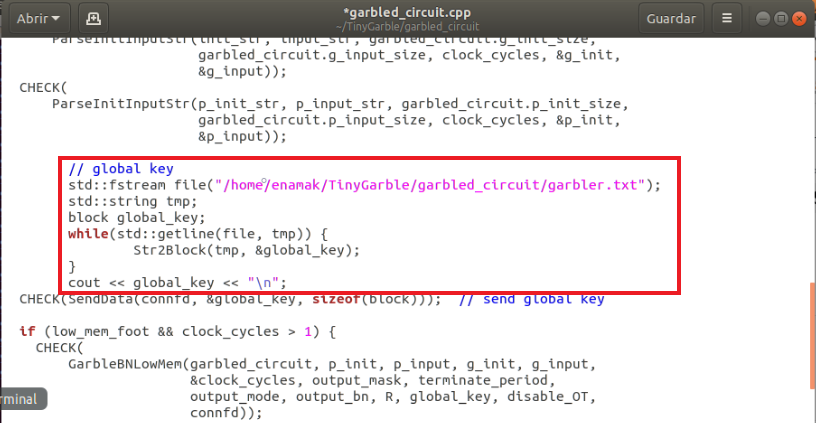
\includegraphics[width=1\textwidth, height=5.5cm]{./sdf/secure_multiparty_computation/figures/key_file.png}
    \caption{Reading Garbler's key from a file.}\label{fig:key_file}
\end{figure}

The figure above is showing a piece of the modified GarbleStr function, the same would have to be done at the EvaluatorStr function with the respective path for the evaluator keys. The absolute(starting from the root) path has to be given. "\#Include <fstream>" is also needed at the top of the file.

To apply any changes made to the file, go to TinyGarble/bin and run the "make" command.

\newpage

\subsubsection{Usage}

\begin{figure}[H]
	\centering
	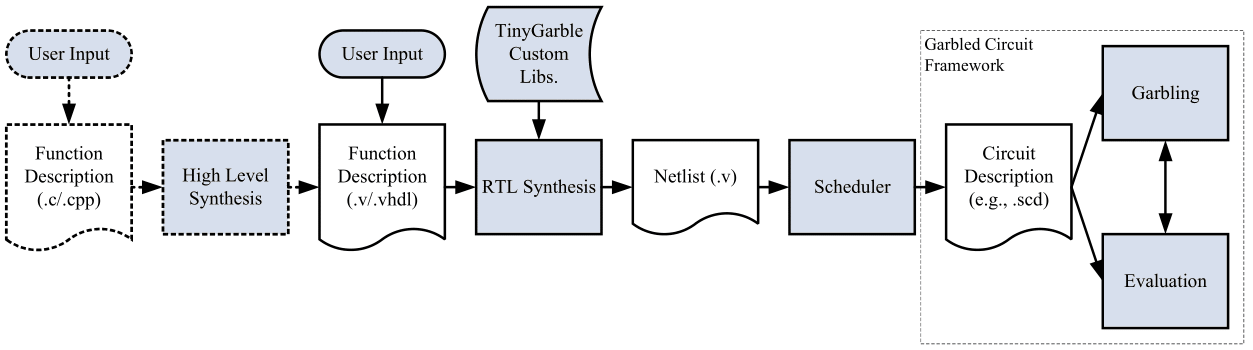
\includegraphics[width=1\textwidth, height=3cm]{./sdf/secure_multiparty_computation/figures/tiny_garble_flow.png}
    \caption{TinyGarble Global Flow\cite{Songhori}}\label{fig:tinygarble_flow}
\end{figure}

Following TinyGarble's global flow showed on the image above, it's possible to see that a C/C++ or Hardware Design Language (HDL) input is necessary. The former is slightly worse in terms of performance, since it needs an extra step of synthesis, with the help of a High Level Synthesis (HLS) tool, like Spart or Xilinx Vivado for C, to compile the C/C++ file into HDL, causing the end SCD file to have more logical gates than when using HDL input directly.

When writting the input file, some attention to the circuit's ports is needed, since TinyGarble's V2SCD (Netlist Verilog to SCD converter) accepts netlist files with a special format. 
Below are the ports that can be used and what they represent.

\begin{itemize}  
\item clk: clock cycle
\item rst: active high reset
\item g\_init: garbler's initial values (read at the first clock)
\item e\_init: evaluator's initial values (read at the first clock)
\item g\_input: garbler's input (read at every clock)
\item e\_input: evaluator's input (read at every clock)
\item o: output
\end{itemize}

Below it's an example of an and\_gate written in verilog with the format above.

\begin{lstlisting}[caption={and\_gate.v}, language=Verilog, captionpos=b] 
module and_gate (input g_input, e_input, output o);
	assign o = g_input & e_input;
endmodule
\end{lstlisting}

If the file is written in VHDL instead, it has to be translated to Verilog with the tool mentioned before, vhd2vl, since the next step needs a Verilog file.

\begin{lstlisting}[caption={Translation of VHDL file into Verilog}, language=bash, captionpos=b] 
$ vhd2vl and_gate.vhd and_gate.v	
\end{lstlisting}

This next step requires the RTL Synthesis tool mentioned before, Yosys, in order to compile the RTL Verilog file into a Netlist Verilog File. 
Using TinyGarble's custom library, "asic\_cell\_extended.lib", located at TinyGarble/ciruit\_synthesis/lib/, and assuming that the Verilog file is located at a folder named "circuits", the compilation can be done with the following instructions:

\begin{lstlisting}[caption={Yosys instructions to compile the HDL file to a Netlist file}, language=bash, captionpos=b] 
$ ./yosys
yosys> read_verilog circuits/and_gate.v
yosys> hierarchy -check -top and_gate
yosys> proc; opt; memory; opt; fsm; opt; techmap; opt;
yosys> abc -liberty TinyGarble/circuit_synthesis/lib/
asic_cell_extended.lib
yosys> clean
yosys> write_verilog circuits/and_gate_netlist.v
yosys> exit					
\end{lstlisting}

Following these, the Netlist file below should be generated.

\begin{lstlisting}[caption={and\_gate\_netlist.v}, language=Verilog, captionpos=b] 
(* top =  1  *)
(* src = "and.v:1" *)
module and_gate( g_input,  e_input, o);
  (* src = "and.v:2" *)
  input g_input;
  (* src = "and.v:2" *)
  input e_input;
  (* src = "and.v:3" *)
  output o;
  AND _0_ (
    .A(e_input),
    .B(g_input),
    .Z(o)
  );
endmodule
\end{lstlisting}

For some unkown reason, the output file has some noticeably weird lines, starting with "(*", that will cause Segmentation Fault error in the next step if not removed.
After removing those lines, the Netlist file can be converted into a SCD file with the instruction below:

\begin{lstlisting}[caption={Installation of Yosys-abc}, language=bash, captionpos=b] 
$ ./TinyGarble/bin/scd/V2SCD_Main -i circuits/and_gate_netlist.v 
-o circuits/and_gate_scd.scd		
\end{lstlisting}

\newpage

The SCD file can now be executed by both parties, "Alice" and "Bob", as shown on the upper terminal and lower terminal of the following images, respectively.
For this examples the SCD file was located at TinyGarble/bin/garbled\_circuits, same directory where the instructions were executed.

\begin{figure}[H]
	\centering
	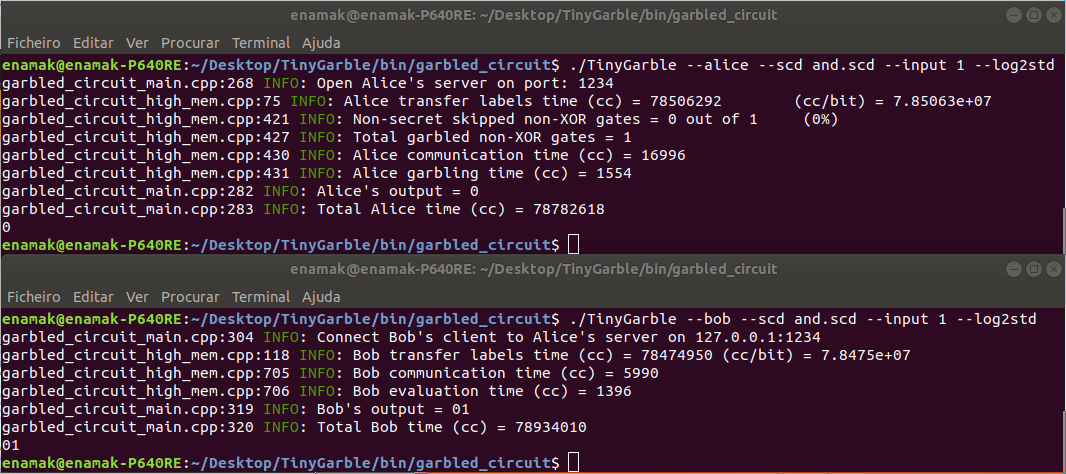
\includegraphics[width=1\textwidth, height=7cm]{./sdf/secure_multiparty_computation/figures/tinygarble_and_a.png}
    \caption{"And" function executed by Alice and Bob, with inputs 1 and 1, respectively}\label{fig:tinygarble_and_a}
\end{figure}

\begin{figure}[H]
	\centering
	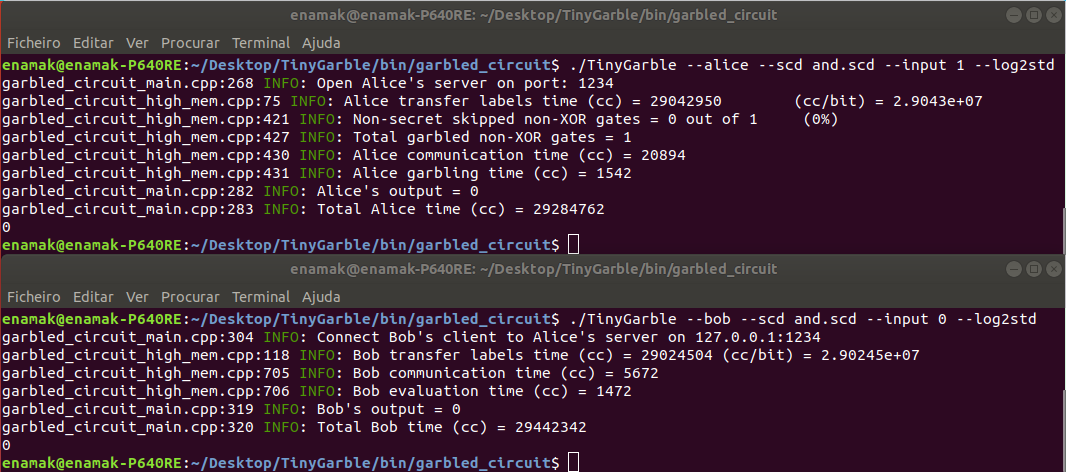
\includegraphics[width=1\textwidth, height=7cm]{./sdf/secure_multiparty_computation/figures/tinygarble_and_b.png}
    \caption{"And" function executed by Alice and Bob, with inputs 1 and 0, respectively}\label{fig:tinygarble_and_b}
\end{figure}

The input is written in hexadecimal, and the log2std option is to show info of the computation on the terminal instead of creating a log file.

\begin{figure}[H]
	\centering
	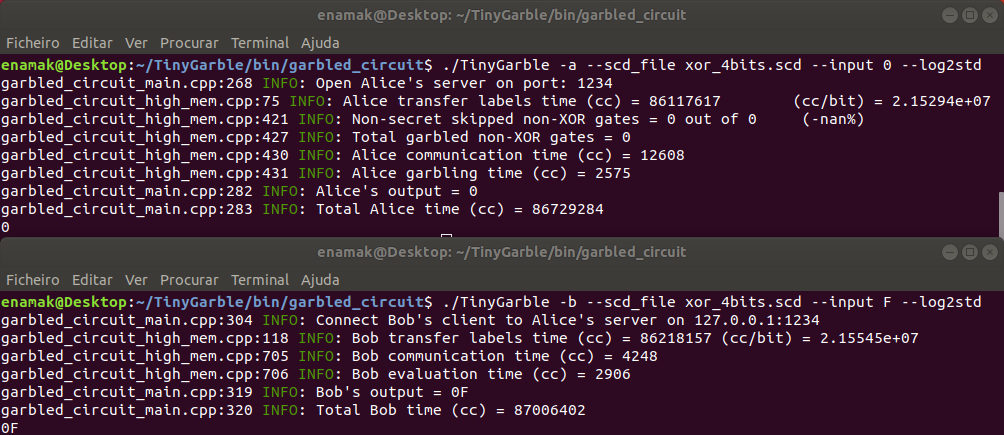
\includegraphics[width=1\textwidth, height=7cm]{./sdf/secure_multiparty_computation/figures/tinygarble_xor_4bits_b.png}
    \caption{"Xor" function with 4 bits, executed by Alice and Bob, with inputs 0 and F, respectively}\label{fig:tinygarble_xor_b}
\end{figure}

\begin{figure}[H]
	\centering
	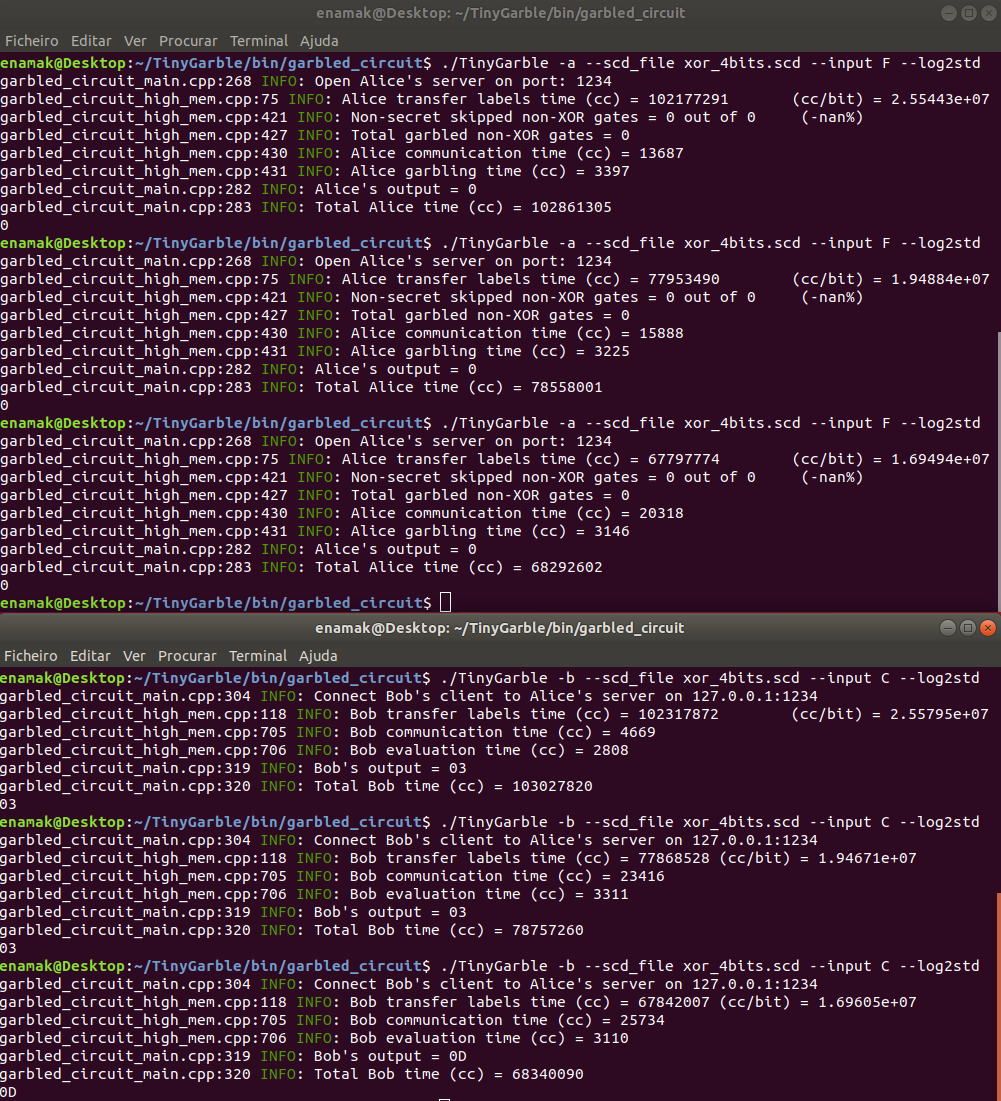
\includegraphics[width=1\textwidth, height=14cm]{./sdf/secure_multiparty_computation/figures/tinygarble_xor_4bits_a.png}
    \caption{"Xor" function with 4 bits, executed by Alice and Bob, with inputs F and C, respectively}\label{fig:tinygarble_xor_a}
\end{figure}


% bibliographic references for the section ----------------------------
\clearpage
\printbibliography[heading=subbibliography]
\end{refsection}
\addcontentsline{toc}{subsection}{Bibliography}
\cleardoublepage
% -------------------------------------------------------------------- 
